\documentclass[twocolumn]{article}
\usepackage{enumitem}
\usepackage[margin=0.75in]{geometry}
\usepackage{graphicx}
\usepackage[hidelinks]{hyperref}
\usepackage{multicol}


\title{Killerbeez: Fuzzing Framework to Bring Together the State of the Art}
\author{Adam Nichols, Ian Bridges, Benjamin Lipton, Jeff Stewart, Tomas Tillery \\
GRIMM\\
\{adam,ian,ben,jeffball,tomas\}@grimm-co.com}
\date{Published: 04 DEC 2018}

% TODO: Make sure we are consistent with our capitalization.  E.g. if we're
%       going to make Driver a proper noun so it is clear that we're talking
%       about it in our domain specific definition, we need to do so
%       consistently.  If not, we need to consistently spell it with a lower
%       case "d"
% TODO: We should be saying seed inputs, not seed files.
% TODO: We should be saying executable instead of binary.
% TODO: Maybe it's be better to refer to the target software instead of target
%       application. Saying "application" is confusing when using Killerbeez to
%       do kernel fuzzing; software covered both cases
% TODO: Remove most/all instances of first person voice (we, us, our, etc.)
% TODO: Ensure all acronyms we use are expanded on first use
\def\AFL{\renewcommand\AFL{AFL}American Fuzzy Lop (AFL)}
\def\COM{\renewcommand\COM{COM}Common Object Model (COM)}
\def\BOINC{\renewcommand\BOINC{BOINC}Berkeley Open Infrastructure for Network Computing (BOINC)}
\def\BTS{\renewcommand\BTS{BTS}Branch Trace Store (BTS)}
\def\GUI{\renewcommand\GUI{GUI}Graphical User Interface (GUI)}
\def\IPC{\renewcommand\IPC{IPC}Interprocess Comunication (IPC)}
\def\IPT{\renewcommand\IPT{IPT}Intel Processor Trace (IPT)}
\def\TNT{\renewcommand\TNT{TNT}Taken Not Taken (TNT)}
\def\TIP{\renewcommand\TIP{TIP}Target IP (TIP)}

\begin{document}
% Heading for the first page has the title, author(s) and date
\maketitle


\textbf{\textit{Abstract}}:
The trend of people increasingly relying on software has continued for
several decades and shows no sign of abating. Businesses rely on Windows and
the applications which run on it, servers are typically some type of UNIX
system, and Apple computers are gaining popularity as of late. The desire is
for these to be stable and resilient to attack, which drives the need to find
software errors which compromise these systems. Many improvements have been
made in the field of software testing, with one of the popular ones being fuzz
testing, or fuzzing for short.  Unfortunately the implementation details make
it difficult to compare or combine different methods, while others are only
available for specific operating systems, or limited to cases where source
code is available.  Killerbeez is intended to pull these technologies together
and get them to interoperate. It is scalable, supports multiple operating
systems, is extensible and will have support for testing both kernel as well
as user space applications. The goal is to be able to measure the effectiveness
of various fuzzing techniques in a variety of situations so the optimal
solution can be applied. 


\section{Introduction} \label{Introduction}
Over the past few years, coverage-guided fuzzing has become a popular way to
find software and hardware vulnerabilities due to advances in publicly
available tools such as \AFL{}\cite{afl} and its derivatives.\cite{vanhauser} Many
fuzzers have ``trophy cases'' consisting of a list of bugs known to be found with that tool to
demonstrate their effectiveness against real-world applications.  However, most
tools are primarily focused on finding bugs in open source, command line Linux
software which reads input from files or standard input. While there has been some
exploration to get \AFL{} working on other operating
systems\cite{aflosx,winafl} as well as supporting network
input,\cite{netafl,preeny} these features are often omitted.

Most of the published improvements over the original version of \AFL{} are
implemented as forks of
\AFL{}.\cite{aflfast,aflgo,fairfuzz,perffuzz,pythia,collafl}
Thus the enhancements are mutually exclusive, short of embarking on a
development effort to review the modifications and merge the forks back
together, manually resolving any conflicts and incompatibilities.  The issue
of incompatibility is not limited to projects which are modified versions of
\AFL{}. Mixing and matching features from various tools requires a significant
amount of effort. Using a tool against a type of software it has never been
used against before, such as using a Linux kernel fuzzer against another
operating system, can find a large number of bugs\cite{anton}.  However, in practice, security
professionals rarely have the amount of time to invest to get the tools working
together, or working in other contexts.

We present Killerbeez, a fuzzing framework which brings together many of the
various security analysis tools so they can be used together.  Killerbeez
supports multiple operating systems, can handle target applications with or
without source code, and software with a \GUI{}.
Furthermore, the input mutation algorithms, instrumentation, seed selection
algorithms, and methods for feeding input data to the target are all easily
interchangeable via modular components.  This modularity enables two
properties (1) easily mixing and matching
tactics from different researchers and (2) implementing new algorithms easily.
Finally, Killerbeez is scalable, using \BOINC{}\cite{boinc} to distribute work
to multiple nodes from a central server.

Our contributions include:
\begin{enumerate}[noitemsep]
\item An \API{} combining the different components of a fuzzer in a pluggable (modular) way to allow for extensibility
\item A collection of existing fuzzers modified to use the \API{}
\item A method for automatically determining which libraries are likely to
	cause a crash, so those can be targeted while fuzzing
\item A technique for quickly utilizing \IPT{} trace information to identify unique code traces while fuzzing
\item Ability to automatically filter out trace data related to non-deterministic code
\end{enumerate}


\section{Background} \label{Background}
There are a huge number of fuzzing tools\cite{afl,aflosx,winafl,peach22,syzkaller,ossfuzz,driller,radamsa,ni,zzuf,synfuzz,brundlefuzz,honggfuzz,kafl,vuzzer,boofuzz} which are publicly available, many of
which are very useful on real-world binaries.
However, each tool
typically only handles one very specific use case or contains other real-world limitations, and most are not designed to scale
out.  For instance, there are a number of fuzzers targeting kernel system calls\cite{syzkaller,trinity,kafl,osxfuzz}, others for
fuzzing \IOCTLs{}\cite{ioctlfuzzer,ioctlbf}, and others for fuzzing userland Linux targets that only effectively work with
command line programs written in C-like languages\cite{afl}.  Some only function with
source code, only work on 32-bit Linux\cite{vuzzer}, or require users to manually specify
the data format which the target is
expecting.\cite{peach,boofuzz}  Finally, there is a category of tools which work amazingly well
on toy programs but do not work on production software due to bugs or lack of
support for features such as multithreading.\cite{grimmdriller,angrissues}

Lack of compatibility with production software is typically not viewed as an issue in academic work, as the problem to address can be
scoped based on the tools that are available; one may assume that the problem can
be solved in other situations, but leave the proof for future work.  The researchers
are typically correct in their assumption, however practitioners need tools
that work in practice, not theoretical solutions.

In industry, the situation is dictated by the target software,
and there is often not a choice as to what language it is
written in, whether source code is available, what operating system it runs
on, or which CPU architectures it supports. This leaves the security
professional to choose between the limited set of tools that can handle the specific requirements of their target, many of which will
turn out to be mutually exclusive. This lack of available tools also creates a new problem, as a common
response to this dilemma is to put together a custom tool which meets their
needs, and to do so in the shortest amount of time possible.  Furthermore,
this results in the same code being re-written for different platforms, or
sometimes for the same platform simply because the security professional was
unaware of existing implementations.  The adapted tool will probably
contain some of the same bugs and limitations that were in the initial
version of the existing tool, which may or may not get fixed before it is
abandoned.

In short, while that state of security research is advancing rapidly, the
tools to bring their benefits to life are sorely lacking.  Though there are some
fuzzing projects which come close, such as OSS-Fuzz,\cite{ossfuzz} there
are not any fuzzing tools which are freely available, work on closed source applications,
are easily extendable,
can be run in a distributed manner, and run against Windows, Linux, and macOS applications.


% The overview describes what components exist (driver, mutator, manager, etc.)
% and why. Examples are provided as needed, but just enough to cover the
% concepts.
\section{Killerbeez Overview} \label{Killerbeez Overview}
The core components of Killerbeez can be split into two logical categories
of orchestration and handling interactions with the target\footnote{Software under test is referred to as the ``target.''}
program.  The former refers to decisions such as what
inputs to use as seed data,\footnote{Initial inputs which will be modified
are referred to as ``seeds.''} which mutation algorithms to use, how to minimize
the input corpus and other decisions which are best left to a central
controller.  The latter category contains actions such as launching the target;
feeding the target input data; tracking code coverage; determining when the target is
done processing the input; and reporting whether the target crashed, froze due
to something like an infinite loop, or executed new portions of code.

\subsection{Orchestration}
Killerbeez coordinates the entire distributed fuzzing
campaign. The orchestration tasks are handled by the Killerbeez ``manager,''
which runs on a central server. After some initial configuration to specify
targets and strategies, the manager decides what jobs to schedule next.
It tracks targets available for fuzzing, selects which tools to
use and how to configure them, manages the corpus of inputs by removing
less interesting ones, and dispatches jobs to worker nodes to be executed.  It also
provides a \REST{} \API{} that allows a researcher to trigger actions and
extract results manually, or to integrate an external system that
does so autonomously. The components of the manager are depicted in Figure
\ref{fig:Killerbeez-server}.

\begin{figure*}[!ht]
\centering
\includegraphics[width=\textwidth]{KILLERBEEZ_Server_Architecture.png}
\caption{Killerbeez Server Architecture}
\label{fig:Killerbeez-server}
\end{figure*}

\subsubsection{Work Distribution}
The most basic role of the manager is to provide an interface for queuing tasks
to be executed on worker nodes and processing the results. A \BOINC{} server is
used to transmit the work to nodes and receive results. The manager provides a
layer on top of \BOINC{} that understands Killerbeez-specific parameters such as
the mutator and instrumentation to use, making it simple to submit jobs to
\BOINC{} that run the fuzzer with an appropriate command line. Jobs
submitted via the manager also automatically set up Killerbeez and the target
software, so the worker nodes are not required to have any special software
installed besides the off-the-shelf \BOINC{} client.

When jobs complete, the manager uses the \BOINC{} ``assimilator'' interface to
collect the results and update the manager's database. The information inserted
includes not only the direct output of the fuzzer (new inputs that cause new
paths in the binary to be hit) but metadata about the job as well. This metadata
could include the average execution time of the binary (to help choose
parameters that execute faster), the final instrumentation state from fuzzing
(to help the next job find fewer duplicate paths), and various other statistics.

Because the manager is not responsible for running the target application, it
does not need to run on the same platform as the target.  Thus, it can run on Linux while
serving work to be executed by Windows or macOS machines.

\subsubsection{Integration}
The manager provides a \REST{} \API{}, which allows clients
to access and configure seed data, fuzzing targets, and low-level metadata
produced during fuzzing.
This will enable future enhancements to be made by taking advantage of
external tools, such as
using a test case generator to produce new seed data. Another planned integration
is to use Driller\cite{driller} to generate program inputs which reach
code which has not yet been reached by mutation.

The \REST{} \API{} is also used for some of the manager's built-in
functionality. The campaign manager, the component that plans new jobs to
execute, uses the \REST{} \API{} to gather data and submit the resulting job.
The corpus minimization uses the \REST{} \API{} to obtain execution traces and
modify the working set of seed values. Accessing data via the \REST{} \API{}
allows these components to be less coupled with the internals of the manager,
enabling them to run as standalone processes. Figure
\ref{fig:Killerbeez-integrations} shows how the \REST{} \API{} enables
integration with various tools.

\subsubsection{Tracing and Corpus Minimization} \label{Corpus Minimization}
Killerbeez also introduces the idea of obtaining detailed information about
execution for each input which has a unique code path.  This is typically
not done by other fuzzers, as obtaining a full trace is much more overhead than
the lightweight instrumentation that \AFL{} or Honggfuzz use. During
normal fuzzing, Killerbeez will generally use lightweight methods of tracking
execution. However, having a full trace is useful when minimizing the seed corpus
and determining which seeds should be weighted more heavily. This concept has
been encapsulated in the tracer module.

Each time an input
is found which hits a new code path, a tracer job can be added via the manager.
This job will be executed by a \BOINC{} client, just like any other fuzzing job.
The results will include full trace data, which will be stored in the manager's
database.  The data can be retrieved via the \REST{} \API{}, enabling a ``corpus
minimizer'' tool to explore the paths covered by the current input corpus and
remove inputs that are redundant. More
information about the tracer and corpus minimizer can be found in section
\ref{Tracer}.

\subsubsection{Work Generation}
The manager is also responsible for deciding what work should be performed next.
The component that does this is called the ``campaign manager,'' and it consists
of several pluggable modules that work together to generate jobs. For
jobs that run the killerbeez fuzzer, the seed selector module specifies an
algorithm for choosing the most interesting input to use as a starting point for
fuzzing, while the job parameter selector module determines parameters like the
mutator to use for the job or the instrumentation options. It is also possible
to integrate tools besides the fuzzer into the job system, such as Driller or
the tracer. The job type selector module is responsible for choosing which of
these tools is currently needed most. The modules can use the \REST{} \API{} to
query any of the metadata recorded in the database to make their decisions.

The manager can choose the amount of work done per job by specifying things like the
number of fuzz iterations, so by scheduling larger jobs it should be able to scale up to a very large number
of clients, allowing a substantial amount of
work to get done with a minimal amount of coordination and network overhead.
However, if the manager becomes a bottleneck, multiple
manager servers could be set up and the \REST{} \API{} interface used to share
information between them.

\begin{figure*}[!ht]
\centering
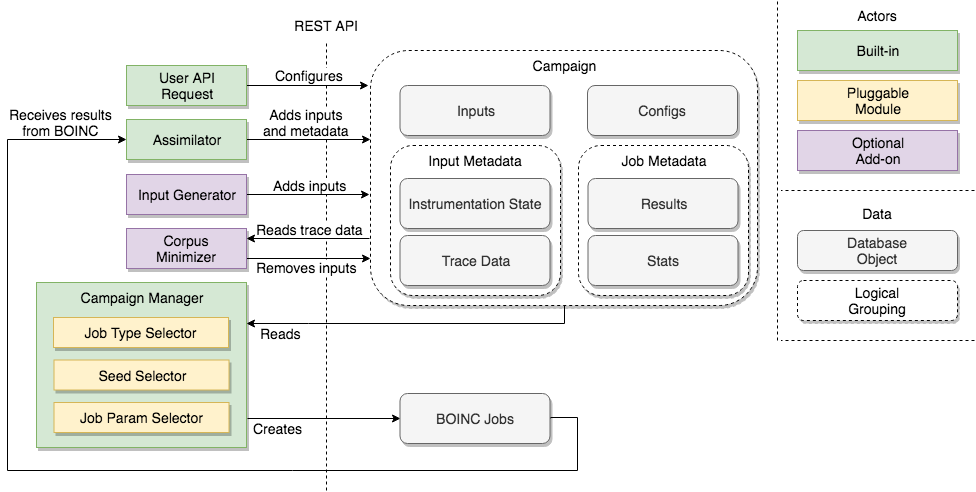
\includegraphics[width=\textwidth]{KILLERBEEZ_Integrations.png}
\caption{Killerbeez Integration with External Tools}
\label{fig:Killerbeez-integrations}
\end{figure*}


\subsection{Preparation}  \label{Preparation Overview}
There is a preparation phase of fuzzing workflows which is often overlooked or
dismissed, that includes setting up the target software and deciding specific
fuzzing parameters. This occurs before any real fuzzing begins and includes
things such as compiling the target, possibly with a specific compiler or
compiler flags, determining what options should be enabled in the target
software, deciding which portions of the code should be tracked for code
coverage, and specifying how to deal with non-deterministic code.

The compilation step is driven by the type of instrumentation chosen,
which is typically just a matter of choosing the option with the lowest
performance penalty. Instrumentation does not need to be added at compile
time, but it is added here when possible, as it reduces the overhead at runtime.
What options to enable in the target software is target specific and
subjective.  It depends on the higher level goals.  If the goal is to find a
vulnerability with wide applicability, choose default options. If it is to test
out a specific feature, disable everything except that option. If it is just to
find any bug in any configuration, enable everything.  While these are
important questions, the most interesting decision is what to track in terms of
code coverage, and how to deal with non-deterministic code.

The solution \AFL{} uses is to require the user to manually determine which code
in the target to instrument. \AFL{} requires the user compile the target library
or executable with a special instrumenting compiler. Alternatively, \AFL{} can
use a modified version of QEMU while fuzzing to instrument all of the libraries
used by a target at run-time.  As expected, instrumenting all of the libraries
has a higher overhead than only instrumenting a few specific modules. Killerbeez
improves on this by including a tool
called the ``Picker'' which automatically determines which libraries should be
instrumented.  The algorithm for doing so is described in section \ref{Picker}.

One important detail is that the picker can not operate effectively when the
target does not have deterministic execution.  If feeding the same file into
the application multiple times results in different code being executed, this
is a problem, not only for the Picker, but also for code coverage in general.
\AFL{} does not deal with this problem directly, but it does alert the user to
the fact that the target is non-deterministic. The user can then do things like
hijack calls to functions such as \texttt{srand()} which intentionally introduces
randomness. This is often done for applications which employ cryptography for
initialization vectors and nonces. Under command line Linux applications, this
works fairly well.  On GUI applications in Windows, it does not work as well.
There are system calls in Windows which occasionally fail for no apparent reason. This
should not be a problem for the target software, as it should be checking the return code to
detect and handle this appropriately.  However, when this happens it has the
side effect of making the fuzzer misinterpret the new code coverage to think an input was interesting when it was
not.  The details of how non-determinism is handled in Killerbeez are also described in
section \ref{Picker}.

\subsection{Execution}
Execution is handled by the client fuzzer program, which is aptly named ``fuzzer.''
This can be run manually from the command line, however it is typically run by
the manager, via a \BOINC{} client.  In either case, the fuzzer is responsible
for running the target, feeding it input data, tracking code
coverage, detecting crashes, and dealing with user interaction such as dialog
boxes.

\begin{figure*}[!ht]
\centering
\includegraphics[width=\textwidth]{killerbeez-high-level-block-diagrams.png}
\caption{Killerbeez Fuzzer Overview}
\label{fig:Killerbeez-fuzzer-overview}
\end{figure*}

The fuzzer consists of glue code that combines together various
modules, which is where all the interesting things occur. The purpose of
the Driver, Mutator and Instrumentation modules used in the fuzzer are covered in sections
\ref{Driver Overview}, \ref{Mutator Overview}, and
\ref{Instrumentation Overview}, respectively.  The relationships between these components are depicted in Figure \ref{fig:Killerbeez-fuzzer-overview}. The modules which currently
exist and how they work are covered in the \nameref{Implementation}
section.

The same code base is used on Windows, Linux and macOS to enable as much code
re-use as possible.  Most of the mutators are shared among all platforms.
Some of the instrumentation and driver\footnote{
``driver'' refers to driver modules, not operating system drivers.}
modules contain platform specific and sometimes target specific code.

\subsubsection{Driver} \label{Driver Overview}
Killerbeez offers drivers, which are target-specific wrappers that abstract
away the concept of loading data into a target and enable finer
definition of the failure modes of a particular piece of software. While
typical fuzzers look for crashes and hangs, specifically-written drivers can
have more context about a given fuzz target.  Better understanding of the fuzz
target's behavior means that Killerbeez can make better-informed decisions
about the status of a target after a particular input, and it can terminate or
classify the result of a particular input more quickly than waiting for a
timeout.

First, the driver module is responsible for feeding inputs to a target.  This
is a departure from most fuzzers, which only work for one type of input.  In
the case of AFL, the input is a file or stdin (which is also a file under
UNIX).  Syzkaller\cite{syzkaller}, on the other hand, uses only system calls.
Each tool then has to implement their own mutation algorithms, code coverage,
results collection and so forth. Drivers enable Killerbeez to reuse all of
these components and select how to interact with the target by simply selecting
the appropriate driver.  Abstracting this away allows for more exotic use
cases, such as fuzzing \IOCTLs{}, network servers, network clients, \IPC{} such as
Mach Messages, XPC, Distributed Objects, \COM{}, and others, all with minimal
effort.

The second thing drivers are responsible for is dealing with any target
specific issues, such as handling GUI interactions.  For example, if a PDF file
with a malformed header is given to a PDF reader application, it typically will
pop up a dialog box indicating that the file is corrupt. Fuzzers such as
Honggfuzz or WinAFL would wait until a timeout expires.\footnote{WinAFL can
exit at the end of a function, but dialog boxes tend to prevent that function
from returning in practice.} This results in all executions which hit this code
path to appear as a hung process.  In Killerbeez, a driver could be written for
the specific PDF reader which monitors the application for dialog boxes,
detects when dialog boxes appear, analyzes the text of the dialog box and
determines that the status is a clean exit rather than a hang.  This would allow
the fuzzer to move on to the next input more quickly, as it would know the
input is done being processed and would not need to wait the full timeout
period.  It also helps discern between a hang, which may indicate a denial of
service vulnerability such as an infinite loop, and an error which is handled
in the expected manner. For another example, see the Windows Media Player
driver in section \ref{Driver}.

Many of the drivers will work on many fuzzing targets in a particular category.
Targets which accept input from the network, are handled by the Network Server
driver module, programs which open a file are generally handled by the file
driver and so forth.  Other drivers can be written to handle things which are
specific to particular pieces of software.  Some targets will handle opening files
differently if opened via double clicking an icon as compared to using the open
option from the file menu. Other examples include error message analysis to
determine if the system should move on to the next input, or if it should click
``OK'' and continue (e.g. in the event of a warning message).

\subsubsection{Mutator} \label{Mutator Overview}
Killerbeez also implements ``mutators,'' which are abstractions on modifying
program input. They decide where to modify bytes in the input data, and how
to modify them.

Killerbeez uses a selection of user-selectable mutators. Parameters are passed
to the mutator module via the driver, which control the operation of the
mutator. For example, the bit flip mutator flips a parametrized number of bits
throughout the entire input, one at a time.

Modular mutators also enable trivial combination of different approaches. Using
the multipart mutator, different mutators can be applied to different parts of
the input. This is required for efficiently fuzzing network protocols, as it is
often desirable to not mutate the initial packets as they may include a handshake or
authentication.  Any mutation to this section would prevent the majority of code from being
executed, as the target software would execute an error path instead. It can
also be used to ensure that the first few bytes in a file are not modified so
the file will still be recognized as being the correct file type.


\subsubsection{Instrumentation} \label{Instrumentation Overview}
Instrumentation modules are responsible for tracking program execution and
determining if an input has caused the target program to execute new code. How it does this,
and what level of granularity is used, are questions left to the module author.
There is an \IPT{} instrumentation module which is very high resolution.
If a loop somewhere in the target is executed 178 times instead of 177
times, it will detect this as a new code path, as the state explored is
different than what was seen before.  The \AFL{} instrumentation module, on the
other hand, would not consider this to be an input which causes the execution of new code.
The \AFL{} instrumentation module uses a bucketing system that groups executions of the same
code and considers anything which executes a portion of code 128-255 times to
be equivalent.

Sometimes instrumentation modules need to interface with kernel drivers, which are
implemented differently on different operating systems. For instance, the \IPT{}
instrumentation module uses the perf subsystem on Linux, which is not available
on macOS or Windows. Other instrumentation technologies, such as Intel's
Pin,\cite{pin} have a very similar interface across different operating
systems, which means more of the code in the instrumentation module can be
re-used, simply using \#ifdef directives if there are portions which are
specific to a particular operating system.


% The implementation goes over each component in detail to showcase what we
% have available so far.
\section{Implementation} \label{Implementation}
Killerbeez is an interoperable fuzzing architecture that is
environment- and platform-independent. It consists of driver, instrumentation,
and mutator modules on the client side, a tracer which obtains accurate code
coverage and a picker which determines which code should be instrumented.
Scalability is achieved by using a \BOINC{} server to allow multiple client
nodes to fuzz in parallel.  Clients simply obtain work from and return results
to the server.

While there are some novel improvements in Killerbeez,
the primary benefit is getting many existing tools to work
together and run on new platforms.  Each tool pulled into Killerbeez was the best in class on its own, but
when combined with others, the value is more than the sum of its parts.

\subsection{Driver} \label{Driver}
Driver modules use the mutator module which is passed in to mutate an input,
the instrumentation module to trace the target's execution, and are responsible
for getting the input data into the target.  A simple example is a
file-based driver, which will create a file containing the mutated input and
use the instrumentation module to launch the application in a way that it will
read this file.  This is typically accomplished by passing a filename on the
command line.  For targets which do not have any way to specify the input
on the command line, a custom driver would be required to use keyboard
shortcuts, mouse input, or some other method of getting the input into the
program.

The following drivers have been implemented:
\begin{itemize}[noitemsep]
\item \textbf{File} - for programs that read input from a file
\item \textbf{Stdin} - for programs that read input from standard input
\item \textbf{Network Server} - enables fuzzing server programs
\item \textbf{Network Client} - enables fuzzing client programs
\item \textbf{Windows Media Player} - for Windows Media Player
\end{itemize}

The File and Stdin drivers provide feature parity with \AFL{}, in terms of input
methods. There is nothing particularly novel about these drivers, but they are
an important feature.  Sending malicious files via email is a popular attack
vector, so there is an interest in proactively finding bugs that can be triggered by loading files.

The Network Server and Network Client drivers provide parity with \AFL{} when it
is combined with Preeny.\cite{preeny}  Two drivers are needed, one to establish
a connection to a server, and the other to accept a connection from a
client. These drivers caused the creation of the multipart mutator,
which is covered in more detail in section \ref{Mutator}.

A Windows Media Player (WMP) driver was created to demonstrate how to deal with
a \GUI{} application which does not exit without user interaction. Applications
with a \GUI{} are difficult to fuzz and many fuzzers evade this problem by not
supporting targets with a \GUI{}.  The typical recommendation is to fuzz the library
which does the heavy lifting, or modify the application to not load a \GUI{}.
This does not work well when dealing with closed source applications. A test
harness can be written which calls the undocumented functions in the closed
source library, but there is no guarantee that bugs found will also be present
and reachable in the real application.  This is due to constraints which may
be placed on function arguments in the main application, or that functions are
called in a different order.  While writing a custom harness to test a library
is a good recommendation, it should not be the only option. Thanks to its
modular drivers, Killerbeez can deal with this problem instead of simply avoiding it.

The next issue a driver has to deal with is determining when the target is done
processing the input.
Typically, a fuzzer's execution loop involves mutating input, feeding it to a
target, and then monitoring the target for interesting behavior such as a crash
or a hang, and if it does not exit after the timeout period, it is considered to
be hung.  This works for command line programs which exit immediately after processing
the input, but falls apart when dealing with \GUI{} applications.
Setting a timeout which is too low results in stopping before the
program is finished processing the input, while setting it too high means
wasting time. On top of this, every non-crashing test case is considered
a hang. WinAFL attempts to address these problems by forcing the user to
reverse engineer the target software to identify the function which reads and
processes input data.  This is time consuming, and if there is one function
which reads the data into memory and another function which parses it, this
strategy does not work well. This can sometimes be worked around by going up
a level in the call stack until the function is located which calls both the reading and parsing functions.
However, that function might also be the one which loads the \GUI{}, which means
it may never return. This breaks WinAFL's assumption that there is a function
which reads input data, parses it, and returns, which means it will fail in the
same way fuzzers intended for command line programs will fail: with every test
case being a hang.  The next alternative is to patch the target executable
to exit after parsing. All of these approaches require reversing the target,
and will have varied results depending on the details of the software under test.

The WMP driver, when used with the DynamoRIO instrumentation, uses the same strategy as WinAFL, where a specific function
name or offset needs to be specified and the test is ended when that function returns, however
this is not the only stopping condition. The driver also checks for sound
playing and assumes that if it was able to decode the file and start playing
sound, that the application has finished parsing the input file.
The underlying assumptions are that errors will be in the
code which does the parsing, rather than the code which does the playing, and that all
the parsing is done up front.  This does mean that bugs which require a
significant number of frames will not be found, as the test will conclude
early and kill the application.  This is a conscious trade-off which was made
to speed up the number of executions per second by terminating much earlier than
waiting for the entire clip to
play or the timeout to occur.  While this technique is based on fuzzing Windows Media Player,
it should work on any media playing application. 

\subsection{Mutator} \label{Mutator}
The mutators from Honggfuzz, Radamsa, AFL, and Ni are leveraged by wrapping the
code from these projects to conform to the Killerbeez Mutator API. By
defining an API for the mutators, researchers can modify other
fuzzers to conform to the Killerbeez API and easily swap in the new mutators.

The following mutators have been implemented:
\begin{itemize}[noitemsep]
\item \textbf{arithmetic} - 32-bit arithmetics, both endians. From \AFL{}
\item \textbf{bit flip} - Flips various number of bits (1-32). From \AFL{}
\item \textbf{dictionary} - Inserts or replaces values from a dictionary. From \AFL{}
\item \textbf{havoc} - Runs multiple mutations on a single input. From \AFL{}
\item \textbf{interesting value} - Inserts values which are more likely to trigger
                                   integer overflows or off-by-one errors. From
                                   \AFL{}
\item \textbf{splice} - Splices two input files together. From \AFL{}
\item \textbf{afl} - All of the \AFL{} mutators, run in the same manner as is
                     done in \AFL{}
\item \textbf{honggfuzz} - Mutation algorithm from Honggfuzz\cite{honggfuzz}
\item \textbf{multipart} - Input must be made up of multiple parts, different
                           mutators are applied to different parts of the
                           input. Useful for network protocols where there is
                           a desire to not disrupt the handshake/login
\item \textbf{ni} - Mutation algorithm from Ni\cite{ni}
\item \textbf{nop} - Mutator which does not mutate anything, useful for
                     testing and when combined with the multipart mutator
\item \textbf{radamsa} - Mutator which wraps the Radamsa\cite{radamsa} executable
\item \textbf{zzuf} - Mutation algorithm from zzuf\cite{zzuf}
\end{itemize}

As indicated in the list above, several of the mutators were taken from \AFL{}
and adapted to the Killerbeez API. These have proven to be effective algorithms
and were a solid starting point.

Honggfuzz has a different set of mutators, some of which are similar to those
from \AFL{}, however there are slight variations which should work better
against some targets than others.  Honggfuzz is the only fuzzer to have found a
crtical vulnerability in OpenSSL,\cite{honggfuzz} so clearly it does
something different than the other fuzzers.  Again, the approach was one of pragmatism:
taking the existing techniques and bringing them to new
environments, such as Windows with code coverage capabilities.

The multipart mutator was driven by the network driver and the desire to have
the handshake or authentication section of the input not be mutated, as this
would prevent much of the interesting code from being reached.  The input is
divided into parts and a mutator is run on each part. For any parts which
should not be modified, the ``nop'' mutator, which is described below, is
selected. This allows different mutators to be used on different segments of
the input and the ones which perform the best can be selected more often by the
campaign manager.  The multipart mutator could also be used with a file-based
driver which is multipart aware, allowing different segments of input files to
be defined.  This would enable things such as ensuring a file's magic bytes are
never modified by using the ``nop'' mutator on the first segment.

Aki Helin, the author of Radamsa, also wrote a mutation algorithm called Ni.
This code was adopted with minimal changes to provide more diversity in
mutation methods, and based on Aki's reputation for having novel ideas on how
to mutate inputs.

During development, it quickly became clear that having a mutator which does
not do any mutation would be handy when debugging issues.  This is how the nop
mutator was born. It was later used when the multipart mutator was developed.

Radamsa is a general purpose fuzzer, written in Lisp, which came from the
OUSPG's Protos Genome Project.\cite{genome} It works well against a variety of network
protocols and file formats, and has found dozens of vulnerabilities.  The
radamsa mutator module in Killerbeez is a simple wrapper which feeds data
to the Radamsa executable.  The strategy of using an external process was chosen
to allow the process to be long lived, so Radamsa's internal state can be
updated over the course of many inputs.  The alternative approach, which
other fuzzing projects have taken when adopting Radamsa, is to pull in the \texttt{main()}
function from the C code (which is generated by the Radamsa Lisp code) and
execute \texttt{main()} once per input.\cite{radamsatob}  This is much faster
in terms of execution time, because the function is executed within the context of the
fuzzer process.  This means data does not need to be piped from one process
to another and then back again, however it loses a key value of Radamsa, which
is that it tends to get better as it sees more data. While the implementation
in Killerbeez is slower, and this reflects poorly on the metric of executions
of the target application per second, it is arguably higher quality mutations
in the long run.  There was an effort to get Radamsa compiled on Windows as a
DLL, which was painstakingly implemented, only to find that it was about twice
as slow as using an external process. The cause of this was not immediately
apparent, and the effort was abandoned in favor of developing other features.

Finally there is zzuf, which is yet another application fuzzer, that
primarily targets media players, image viewers and web browsers.  As with
other mutators which were pulled in from other projects, it has found bugs in
production code ranging from audio and video codecs to objdump and nm.

Each of the mutators brings diversity to Killerbeez.  Different authors are
going to frequently have different approaches, and even when the algorithms
are similar, there are frequently implementation details which will vary in
ways which are sometimes important.  Different mutation algorithms will
perform differently on various targets.  The benefit of being able to easily
switch from one to another enables Killerbeez to measure which ones are finding
more inputs which trigger new code execution on different targets and at different points in
the fuzzing process.  A mutator which performs poorly with the initial corpus
of inputs may be the best later when a different section of code is unearthed.

\subsection{Instrumentation} \label{Instrumentation}
Killerbeez uses an instrumentation abstraction, to implement the
feedback-based portion of the fuzzer. Instrumentation monitors code coverage of
the target binary. Feedback-based fuzzing helps expand code
coverage by reducing the input set to only those that reach new code.
This reduces that the likelihood that multiple inputs will be tested that result
in the same code coverage.

The following instrumentation modules have been implemented:
\begin{itemize}[noitemsep]
\item \textbf{Debug} - A na\"ive Windows-only instrumentation that determines the
	result of a round of fuzzing via the Windows Debug API.
\item \textbf{Return Code} - A Linux-only equivalent to the debug instrumentation that
	uses the \texttt{waitpid()} system call to determine the result of a fuzz round.
\item \textbf{DynamoRIO} - An instrumentation that uses the DynamoRIO project\cite{dynamo} to
	determine new code paths discovered in a binary.
\item \textbf{Intel PT} - An instrumentation that uses Hardware-level ``Process Tracing''
\item \textbf{AFL} - An instrumentation injected by a modified version of AFL's compilers (afl-gcc or
	afl-clang-fast), or via running the executable under a modified version of QEMU\cite{qemu}
\end{itemize}

The instrumentation modules monitor, at minimum, whether a process crashed,
exited cleanly, or timed out. More advanced instrumentation modules, such as
DynamoRIO, monitor basic block coverage and can inform the fuzzer of new code paths
taken in a binary.  Instrumentation developers decide what options their
module has and whether they will implement optional features. For example, a
module can do only lightweight tracking, as is done in \AFL{}, or it can
optionally support tracking every
basic block executed and each transition.  If it can do the slower, more
accurate tracing, it is considered to be not only an instrumentation module,
but also a tracer.  How tracers are used is covered more in section
\ref{Tracer}.

The Debug instrumentation is currently a Windows-only instrumentation which
attaches to the target process using the debugging interface and monitors the
process for a crash or clean exit.  It does not track code coverage.
This is used for ``dumb'' fuzzing.  The driving force behind this module was
that there is no reliable way to determine if a process crashed or exited normally
on Windows without debugging it.  Unlike Unix, the return code does not contain this information,
so there is no way to tell the difference between a program that decided to
exit with a non-zero status code to indicate an error, and a crash.

The Return Code instrumentation module is similar to the Debug instrumentation
in that it does not track code coverage. On POSIX operating systems, the return
code of a process is a 32-bit integer.  Only the eight least significant bits
are provided to the shell, but the full value is available from the
\texttt{waitpid()} function and macros such as WIFEXITED and WIFSIGNALED can be used to
discern between a clean exit with a non-zero exit code and an actual crash.

The DynamoRIO instrumentation module is a modified version of the
instrumentation in WinAFL. It requires the user to specify a function which
is responsible for loading and processing the input data. At the end of the
target function, DynamoRIO will kill the process. There is an option to reset
the stack and jump to the beginning of the function again, which may work in
test applications, but does not tend to work in real-world software.  
The typical result is a crash due to global state which is never reset.
This includes things like open file handles, allocated memory, application specific state
information, etc. The target function must be identified outside of
Killerbeez and is typically done manually. By default, an \AFL{}-style bitmap
is generated to track code coverage. The module takes options which allow this
to be changed to obtain a full trace (see section \ref{Tracer} for details on
this feature). Other options include a list of libraries which should be
covered by instrumentation. This allows things like tracking code coverage in acrord32.dll
when fuzzing Adobe Reader.  Tracking code coverage in modules is an important
feature, because the majority of the interesting code is encapsulated in a
DLL and recompiling is not an option. This feature was obtained from the
WinAFL\cite{winafl} project and is not present in the stock version of \AFL{}.

The Intel PT module uses \IPT{} to gather trace information for CPUs which
support \IPT{}. This requires a kernel component to manage \IPT{}, but
the tracing itself is done in hardware with a modest performance overhead. The
current implementation of this instrumentation module only works on Linux, via
the ``perf'' subsystem. Expanding this to support the \IPT{} driver in Windows
is planned in the future. Regardless of operating system,
the output of \IPT{} relevant for tracing execution in fuzzing are the \TNT{} and
\TIP{} packets.  The former tracks ``the direction of direct control branches,''
while the latter records ``the target \IP{} of indirect branches, exceptions,
interrupts and other branches or events.''\cite{intelptmanual}

The \TNT{} packets form a bit stream, while the \TIP{} packets contain a series of
instruction pointer addresses, which may be compressed if the \IP{}'s upper bits match
the previous \IP{} value. However, these two packet types are not synchronized. For example, if there are four
conditional branches, an indirect jump, and then four more conditional branches, \IPT{} will generate
a \TIP{} packet and one byte of \TNT{} packet data with no
information about the order in which the \TIP{} and \TNT{} events occurred.  To make sense of
this data, the executable must be analyzed to determine the order in which to
pull information from the \TNT{} and \TIP{} queues. As this disassembly adds to the performance
overhead, the Intel PT instrumentation module does not do it. Instead it
takes a hash of the entire \TNT{} bit stream and the entire set of \IP{} addresses in the \TIP{} packets.
This does not identify what code was executed, but it does determine if a
different code path was taken, as a different code path would result in
different packet data, and thus a different hash. Because the packet order is
not synchronized between the \TNT{} and \TIP{} streams, hashes are taken of each
stream separately and the pair of hashes are used to identify a particular code path.

The only other public fuzzers known to implement Intel PT based tracing are
Honggfuzz\cite{honggfuzz}, Richard Johnson's modified version of
WinAFL\cite{winaflintelpt}, and kAFL\cite{kafl}. Honggfuzz does full packet decoding using the
Intel's processor trace decoder library\cite{libipt} which incurs a much
higher overhead than the Killerbeez implementation.  Richard's fork of WinAFL
did full packet decoding at one point, but does not seem to use the trace data
at all with the latest commit.\cite{winaflcommit} Instead, there is a comment which says
``FIXME winipt'' and the calls to \texttt{PtTraceProcessStart()} and
\texttt{PtTraceProcessStop()} have been commented out, which implies this is still a
work in progress. kAFL utilizes a custom packet decoder built specifically to
allow efficient parsing of the \IPT{} packets and diassembly of the target
executable.  As such, kAFL's \IPT{} parser is faster than the Intel processor trace
decoder library, but is slower than the approach taken in Killerbeez which
refrains from analyzing the target executable.

Finally, we have the \AFL{} instrumentation module, which is based around the
instrumentation injected at compile time by afl-gcc or the \AFL{}
llvm module. Much of the code was taken directly from \AFL{} and adapted to
conform to the Killerbeez instrumentation API. This module has been tested
with Linux and macOS, but should work on any POSIX operating system.
The injected fork server is a slightly modified version of the
implementation in the \AFL{} project. The forkserver is also used by the
Intel PT module, which splits the ``fork'' and ``run'' actions, as \IPT{} needs
to be initialized between these two steps.  The original AFL implementation
combined these two actions, as they did not have any use case that required
them to be separate.  The \AFL{} instrumentation modules also
implements the persistence mode feature
which is included in \AFL{}.  \AFL{}'s QEMU user mode tracing is also included in Killerbeez,
however this mode only works on Linux as QEMU user mode is only
available there.  QEMU chain caching, which is disabled in \AFL{},
has been enabled in the Killerbeez implementation via the patch made by Andrea Biondo.\cite{qemuspeedup} This patch
to QEMU ensures chains are properly tracked and results in a 3-4x improvement
in performance.

This puts the Killerbeez implementation of the source-based \AFL{}-style
instrumentation equivalent with the original implementation and the QEMU
feature significantly faster, showing the advantages of combining the
innovations of different authors.

\subsection{Tracer} \label{Tracer}
A tracer is an instrumentation module which captures detailed trace
information about exactly which basic blocks were executed, along with the
transitions between them and implements some optional functions in the API
which return this information.  This coverage information is commonly referred
to as nodes and edges.

The DynamoRIO instrumentation module is an example of both a normal
instrumentation module and a tracer. By default, it does lightweight tracing to
obtain the \AFL{}-style bitmap coverage information and returns an error if it
is asked for nodes and edges. The ``edges'' option can be enabled to
switch the module to capture full trace information.
Enabling the more accurate tracing mode has a larger overhead, so it is not
used for every iteration of fuzzing.

As a counterexample, the Intel PT instrumentation module is currently not a
tracer.  Without full \IPT{} packet decoding, it is not possible for this
module to obtain such detailed information.

Any time trace information is found, the assimilator stores it in the manager's
database in a standard format.  This is possible because the APIs which get
nodes and edges require the data to be in a specific format.  Any other trace
data is allowed to be in any format, as it is passed around as an opaque blob
and not consumed by anything other than the instrumentation module which
created it.  Trace data is accessible via the manager's REST API.

The trace data can later be used to reduce the set of seeds to only include the minimum
number of files, or the minimum file size, which hits the maximum amount of
code. The concept of minimizing test corpora while maintaining the maximum code
coverage dates back to at least October of 2008, when Peach Fuzzer version 2.2
was released, which included the minset tool.\cite{peach22}  There are a number
of different algorithms which could be chosen, which is why this is handled by
an optional add-in which can be swapped out at will, as shown in Figure
\ref{fig:Killerbeez-integrations}.

This granular code coverage data can also be used for weighting seeds based on
various algorithms, such as attempting to get to code which is less frequently
covered, or targeting a particular piece of code such as a parser which was
manually identified or a new piece of code which was identified using automated
patch analysis. This would be implemented by the seed selector module from the
campaign manager.  The most basic seed selection algorithm would weight
all of the seeds equally and go through them in a round-robin fashion.

Determining how often to use the tracer is the responsibility of the job
type selector in the campaign manager.  This module has the ability, but
not the obligation, to take node and edge coverage into account.  The simplest
algorithm would never enable the tracer, which would inhibit all other
components from using trace data.

\subsection{Picker} \label{Picker}
Instrumenting all libraries for a real application using a dynamic
instrumentation technology is prohibitively slow. Even when using more
efficient instrumentation methods, there is a desire to minimize the amount of
overhead in instrumentation so more effort can be spent finding bugs instead of
performing bookkeeping operations.  The Picker automatically determines which
libraries should be instrumented so the fuzzer can limit instrumentation to
what is interesting, and omit all the other libraries. For deterministic
code, this comes with a level of certainty that what is instrumented is, in
fact, all of the code which handles the input the fuzzer is sending it. This
step is taken when configuring a target, before any fuzzing begins.

The Picker determines the library to instrument by running through all seed values and instrumenting each
library separately. If the code is never executed, or the coverage is the
same for every input, it implies the library is not important in parsing the
input.  It is possible that the library handles some aspect of the
protocol which was simply never executed by any of the seed inputs, however,
with a diverse set of starting inputs, there can be some confidence that
nothing is omitted for the list of modules to instrument.

Code which is non-deterministic causes problems with the algorithm above.
Tracking down each source of non-determinism and attempting to eliminate it
would be very tedious task. An example of one source of non-determinism was a
call to a graphics libraries failing to allocate a surface object. It is
difficult to know how to remove this type of non-determinism. Every system call
which fails on a regular basis would have to be analyzed, and a decision made
on what to do about it.  Making it always fail may cut off code paths later
which trigger a bug which would be reachable in the program in practice.
Repeatedly making the call until it succeeded may also eliminate code paths
later, plus makes execution slower at best and an infinite loop at worst.

Instead of trying to force the non-deterministic program to behave in a
deterministic fashion, the Picker accepts that the code in question is
going to behave erratically and ignores the execution data related to those
sections of code.  This is done by running the same input through the target
\textit{N} times and finding all of the bytes in the coverage info which
vary. By default, \textit{N} is 10, however it should be large enough that a
significant number of executions do not identify any more bytes where the
execution varied. The correct value for N will vary from one target to another.
The data for Windows Media Player, shown in Figure \ref{fig:picker}, indicates
new non-deterministic code was being found after 325 executions. However, after
10 executions, more than half of the non-deterministic transitions were
identified for each of the four DLLs.

Choosing the number of executions is a trade-off between spending time up front
to get more efficient fuzzing, and getting started more quickly but being less
efficient.  In addition to determining which libraries to instrument, the
identified non-deterministic transitions can be used by some instrumentation
modules in determining if an input caused new code paths to be found.  This is
currently only implemented in the DynamoRIO instrumentation module, but will
likely be implemented in the several of the instrumentation modules listed in
the \nameref{Future Work} section.

\begin{figure*}[htb]
\centering
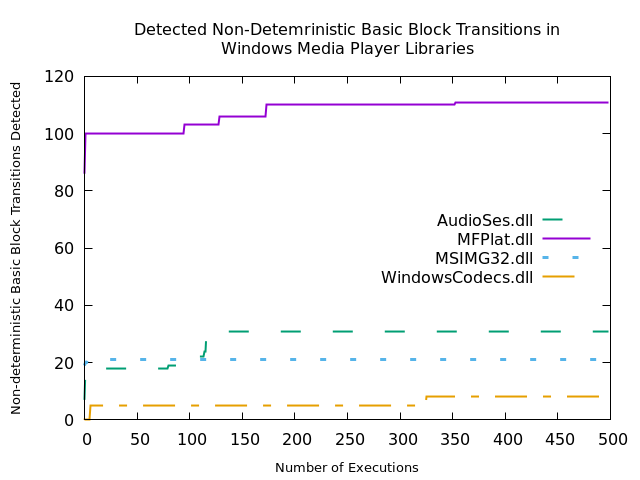
\includegraphics[width=4in]{picker.png}
\caption{Total Non-deterministic Basic Block Transitions Detected per Execution In Windows Media Player Libraries}
\label{fig:picker}
\end{figure*}

The algorithm the Picker uses is not effective with all instrumentation
modules. The Picker uses the instrumentation module which will be used in
practice, and uses the same options for that module. It then operates on
the opaque blob which represents the code coverage information.  It does
this without any knowledge of the internal format.  Anything which uses the
\AFL{}-style bitmap will work fine.  This would include the DynamoRIO and
\AFL{} instrumentation modules. The \IPT{} instrumentation output is the hashes
of the \TNT{} and \TIP{} packets, so any non-determinism will change every byte of
the instrumentation data.  This will cause the Picker to mask out all bytes of
the coverage data, which is not useful. If the Intel PT
instrumentation was also a tracer, it would be capable of using an internal
format which is compatible with the Picker.


%\section{Evaluation} \label{Evaluation}

%\section{Conclusions} \label{Conclusions}

\section{Related Work} \label{Related Work}
There are projects which have addressed some of the aspects covered by Killerbeez
such as platform independence, distributed fuzzing, leveraging existing tools,
and so forth.

Google's OSS-Fuzz\cite{ossfuzz} addresses scalability by running many fuzzers
in parallel, as well as re-using existing code by leveraging tools like
Honggfuzz to handle the actual fuzzing. The core fuzzing component of OSS-Fuzz,
CluserFuzz, is unpublished and therefore unavailable to anyone outside of
Google.  Another difference is that OSS-Fuzz requires source code for the
target software, and also requires that tests be written to integrate it
into the overall system. This adds efficiency, as the test cases can eliminate
code like GUI libraries, which is not the real target of the fuzzing, however
it is unable to test closed source software.

\AFL{}\cite{afl} is an open source fuzzer that uses coverage data and genetic
algorithms to automatically discover interesting test cases in a target.  \AFL{}
was designed to be practical; it has a low overhead, is easy to use, and works
against real-world software. As such, \AFL{} has become one of the most popular
fuzzers and many research projects investigate how to improve \AFL{}. Killerbeez
borrows many features from \AFL{}, such as the compiler and QEMU
instrumentations. While Killerbeez has also borrowed \AFL{}'s mutation strategy,
it does not currently include \AFL{}'s mutations which mutate based on coverage
data. Coverage data is used to avoid wasting time mutating portions of the input
that the target does not process. These mutations will be incorporated into
Killerbeez in the future.  While \AFL{} is a great local fuzzer, it is not
easily distributed and cannot easily manage the fuzzing of more complex targets.

Peach Fuzzer\cite{peach} now supports distributed fuzzing, modular mutators, and
modules for launching apps, is able to do both file and network-based fuzzing,
and does work on closed source applications.  However, the distributed aspect
is only available in the proprietary version of the fuzzer; it does not exist
in the community edition, which is open source. There is also no feedback loop
for code coverage in either edition.  Instead, the input format needs to be
manually described in XML files, as does the model for the program state. To
alleviate this problem, the company behind Peach Fuzzer is willing to sell
access to the definitions they have created.

Honggfuzz\cite{honggfuzz} is an open source fuzzer which runs on Windows, Linux,
macOS, Android, FreeBSD and NetBSD, all using a single code base. It can handle
closed source applications, long-running applications such as servers, and will
automatically use multiple CPU cores to do fuzzing in parallel. Modularity is
achieved by allowing an external program to do the mutation of inputs. While
Honggfuzz scales nicely on a single machine, it does not have any built in
mechanism to utilize multiple machines.  Using Honggfuzz in a larger framework
such as OSS-Fuzz takes care of this limitation.  In fact, Honggfuzz is a fuzzer
which will be likely integrated into Killerbeez in the future, as described in
section \ref{Future Work}. Honggfuzz has more types of instrumentation than any
other fuzzer, including Killerbeez at the time of writing, however none of
these work on Windows. The \BTS{} and \IPT{} instrumentations are only for
Linux, as is the hardware-based counters instrumentation which tracks the
number of instructions and branches which were executed. There is also compile time
instrumentation, but this is only helpful in the case where source code is
available, and it can be compiled by GCC or LLVM.  It is possible to compile
some C/C++ code for windows using LLVM, but anything which requires Microsoft
Visual Studio to be compiled will not have any instrumentation.  Supporting
Windows does not seem to be a priority for Honggfuzz, as it cannot be compiled
natively, but only via Cygwin.

Honggfuzz is a great tool, which is why a modified version of it was created
which can use all of the Killerbeez modules.\cite{honggfuzzgrimm} Section
\ref{Future Work} describes the Linux instrumentation technologies from
Honggfuzz planned for integration with Killerbeez.
If it is feasible to add the ability to use
Killerbeez instrumentation modules, that is another contribution which will be
made to the Honggfuzz project.


% This is where we cover planned expansions, both in terms of additional things
% to pull in, such as grammars which generate test files, Driller style
% integration of symbolic execution, and additional modules for the existing
% components (drivers, instrumentation, etc.).
\section{Future Work} \label{Future Work}
% Summary of the future work
The short term focus will be to pull in existing technologies from other
projects and get them integrated with Killerbeez and running on all the
supported platforms.  There is ample research, tools and techniques available
now which have yet to be applied in different domains. Once the state of the
art has been incorporated, more automation and designing interfaces to pull in
projects which don't fit into the existing modules will be the next priority.

Expanding the coverage of the instrumentation modules so they work on more
operating systems is a high priority. The \IPT{} module currently only works
on Linux, but should be able to work on Windows now that driver support has
improved. The opposite is true for DynamoRIO, which currently works on Windows
but should be able to be ported to run on macOS and Linux without too much
difficulty.  Pulling in more instrumentation technologies such as Intel's PIN,
and Dyninst\cite{dyninst} is also on the list of things to do. Wrapping up the
future enhancements to instrumentation is making more instrumentations aware of
the non-deterministic portions of code which were identified by the Picker.
Currently only the DynamoRIO instrumentation can use this information, but
it should be easy to extend this to all of the \AFL{}-bitmap compatible
instrumentation modules.  This includes the \AFL{} module and the to-be-written
PIN and Dyninst modules.  The \IPT{} module will not be able to use this data
because it does not actually decode the TNT and TIP bitstreams to determine what
code is being executed. Adding real-time parsing would slow down the target
software significantly, however this would still be considered if the benefit
of handling non-deterministic code appears to be worth the additional overhead
which would be incurred.

Expanding the selection of drivers to include the ability to monitor dialog
box pop-ups on Windows is an area of interest. There are already drivers for
the more common input methods, such as files, stdin, and network data, however
these should also be expanded to cover kernel functions via syscalls, drivers
via ioctls, IPC messages, and so forth. This will make Killerbeez be a fuzzer
which can handle not only applications on multiple operating systems, but also
the kernel of multiple operating systems as well.  Currently this is only
theoretically possible with Killerbeez, which is not much help to researchers
in the field. Making it actually possible in practice will be a big step.

The mutation algorithms from several other projects have already been
integrated with Killerbeez, however it is desirable to have the ability
to write mutators in Python.  This will allow pulling in mutators from
projects like BrundleFuzz\cite{brundlefuzz} as well as quickly putting
together a custom mutator without needing to learn as many of the Killerbeez
APIs, nor even needed a compiler.

In addition the aforementioned modules on the client side, there are a number
of algorithms to pull in from academic publications.  This includes the seed
energy rating and power schedules from AFLFast\cite{aflfast} and
AFLGo.\cite{aflgo} FairFuzz presents another seed selection algorithm to bias
seed files toward code segments which are not often executed.\cite{fairfuzz}
The algorithm from the PerfFuzz\cite{perffuzz} paper can be pulled into
Killerbeez to find algorithmic complexity vulnerabilities. The research on
using estimators and extrapolators to determine if a fuzzing campaign should
be stopped, or continue running, can be pulled in from Pythia.\cite{pythia}
Instrumentation modules can be updated to implement the collision resistent
algorithm from CollAFL.\cite{collafl} Angora is also on the list of techniques
to integrate into Killerbeez, however it is at the end of the queue of
improvements due to the fact that it would need to be completely re-implemented
on account of the authors never releasing the code.\cite{angora}

The need to obtain a wide variety of seed values is a weakness of Killerbeez
as well as many other fuzzers. The quality of the starting corpus makes a big
difference of the efficiency of fuzzing.

There are a number of security analysis and even fuzzing tools which do not
fit into mutators, drivers, nor instrumentation modules. This includes input
generation tools, such as Driller\cite{driller} and Synfuzz\cite{synfuzz}.
Integrating Driller will require some code to be written to obtain the target
executable and code coverage information information from the Killerbeez
Manager, run Driller, and add new inputs which will reach new code. All of this
can be accomplished with adding endpoints to the existing REST server. Pulling
in inputs generated with Synfuzz should be even easier, as the only required
REST API which should be required is the ability to add files to the corpus.
Some automation of setting up Synfuzz may also be possible, but it requires
an oracle to determine which inputs are valid or not, which will likely mean
it will need to be set up manually, short of a development which allows
autonomously detecting such oracles and hooking the appropriate functions.


% Not sure if we want to take on the things below or not, but if so they will
% be in the far future.
% Unsolved problems:

% How to choose targets
% Where to get seeds?
%   Search the web, very ad-hoc and manual process
% Avoiding the easy-to-find crashes to get to the more interesting ones
%   Could be done with smarter input generators/mutators & automated static/dynamic analysis
% Targets which include checksums, compression or encryption
%   Typical solution, modify the source/executable to remove those checks


% Room for improvement:

% Detecting non-crashing errors (especially without source code for the target)




\section{References} \label{References}
\renewcommand{\section}[2]{}  % Removes the title thebibliography wants to add
\begin{thebibliography}{99} % two-digit numbers, max

\bibitem{afl}
  Michal Zalewski. % Author
  \textit{American Fuzzy Lop}. % Title
  \url{http://lcamtuf.coredump.cx/afl/}. % URL

\bibitem{vanhauser}
  Marc ``van Hauser'' Heuse.
  \textit{Collection of Patches to AFL}.
  \url{https://github.com/vanhauser-thc/afl-patches/}.

\bibitem{aflosx}
  Ben Nagy.
  \textit{AFL on OSX}.
  \url{https://github.com/bnagy/osx-afl-llvm}.

\bibitem{winafl}
  Ivan Fratric.
  \textit{WinAFL - Fork of AFL for Windows}.
  \url{https://github.com/ivanfratric/winafl}

\bibitem{netafl}
  Maksim Shudrak.
  \textit{winAFL patch to enable network-based apps fuzzing}.
  \url{https://github.com/mxmssh/netafl}

\bibitem{preeny}
  Yan Shoshitaishvili.
  \textit{Preeny: preload libraries for pwning stuff}.
  \url{https://github.com/zardus/preeny}

\bibitem{boinc}
  University of California.
  \textit{Berkeley Open Infrastructure for Network Computing}.
  \url{https://boinc.berkeley.edu/}.

\bibitem{peach22}
  Michael Eddington.
  \textit{Peach Fuzzer version 2.2}.
  \url{https://sourceforge.net/projects/peachfuzz/files/Peach/2.2/}.

\bibitem{aflfast}
  Marcel B\"ohme, Van-Thuan Pham, Abhik Roychoudhury.
  \textit{Coverage-based Greybox Fuzzing as Markov Chain}.
  \url{https://www.comp.nus.edu.sg/~mboehme/paper/CCS16.pdf}.

\bibitem{aflgo}
  Marcel B\"ohme, Van-Thuan Pham, Manh-Dung Nguyen, Abhik Roychoudhury.
  \textit{Directed Greybox Fuzzing}.
  \url{https://mboehme.github.io/paper/CCS17.pdf}.

\bibitem{fairfuzz}
  Caroline Lemieux, Koushik Sen.
  \textit{FairFuzz: Targeting Rare Branches to Rapidly Increase Greybox Fuzz Testing Coverage}.
  \url{https://arxiv.org/pdf/1709.07101.pdf}.

\bibitem{perffuzz}
  Caroline Lemieux, Rohan Padhye, Koushik Sen, Dawn Song.
  \textit{PerfFuzz: automatically generating pathological inputs}.
  \url{https://dl.acm.org/citation.cfm?doid=3213846.3213874}.

\bibitem{pythia}
  Marcel B\"ohme.
  \textit{STADS: Software Testing as Species Discovery}.
  \url{https://mboehme.github.io/paper/TOSEM18.pdf}.

\bibitem{collafl}
  Shuitao Gan, Chao Zhang, Xiaojun Qin, Xuwen Tu, Kang Li, Zhongyu Pei, Zuoning Chen.
  \textit{CollAFL: Path Sensitive Fuzzing}.
  \url{http://chao.100871.net/papers/oakland18.pdf}.

\bibitem{syzkaller}
  Google.
  \textit{syzkaller - kernel fuzzer}.
  \url{https://github.com/google/syzkaller}.

\bibitem{trinity}
  kernelslacker.
  \textit{Trinity - Linux system call fuzzer}.
  \url{https://github.com/kernelslacker/trinity}.

\bibitem{osxfuzz}
  MWR Labs.
  \textit{macOS Kernel Fuzzer}.
  \url{https://github.com/mwrlabs/OSXFuzz}.

\bibitem{ioctlfuzzer}
  eSage Lab.
  \textit{IOCTL Fuzzer}.
  \url{https://github.com/Cr4sh/ioctlfuzzer}.

\bibitem{ioctlbf}
  Jeremy Brun.
  \textit{Windows Kernel Drivers fuzzer}.
  \url{https://github.com/koutto/ioctlbf}.

\bibitem{ossfuzz}
  Google.
  \textit{OSS-Fuzz - Continuous Fuzzing for Open Source Software}.
  \url{https://github.com/google/oss-fuzz}.

\bibitem{driller}
  Nick Stephens, John Grosen, Christopher Salls, Audrey Dutcher, Ruoyu Wang,
  Jacopo Corbetta, Yan Shoshitaishvili, Christopher Kruegel, Giovanni Vigna.
  \textit{Driller: Augmenting Fuzzing Through Selective Symbolic Execution}.
  \url{http://www.cs.ucsb.edu/~chris/research/doc/ndss16_driller.pdf}.

\bibitem{pin}
  Intel Corporation.
  \textit{Pin - A Dynamic Binary Instrumentation Tool}.
  \url{https://software.intel.com/en-us/articles/pin-a-dynamic-binary-instrumentation-tool}.

\bibitem{ni}
  Aki Helin.
  \textit{Ni mutator}.
  \url{https://github.com/aoh/ni}.

\bibitem{radamsa}
  Aki Helin.
  \textit{Radamsa - a general-purpose fuzzer}.
  \url{https://gitlab.com/akihe/radamsa}.

\bibitem{radamsaresults}
  Aki Helin.
  \textit{Radamsa - Some Known Results}.
  \url{https://gitlab.com/akihe/radamsa/blob/master/README.md#some-known-results}.

\bibitem{radamsatob}
  Trail of Bits.
  \textit{Grr Radamsa Modifications}.
  \url{https://github.com/trailofbits/grr/tree/master/third_party/radamsa}.

\bibitem{radamsagrrproblems}
  Aki Helin.
  \textit{Grr Radamsa Modifications Comments}.
  \url{https://gitlab.com/akihe/radamsa/issues/28#note_77242061}.

\bibitem{zzuf}
  Sam Hocevar.
  \textit{zzuf - general purpose fuzzer}.
  \url{https://github.com/samhocevar/zzuf}.

\bibitem{synfuzz}
  Joe Rozner.
  \textit{Synfuzz - re-targetable grammar based test case generation}.
  \url{https://github.com/jrozner/synfuzz}.

\bibitem{dyninst}
  The University of Wisconsin, University of Maryland.
  \textit{DyninstAPI: Tools for binary instrumentation, analysis, and modification}.
  \url{https://dyninst.org/}.

\bibitem{brundlefuzz}
  Carlos Garcia Prado.
  \textit{BrundleFuzz - a distributed fuzzer for Windows and Linux using dynamic binary instrumentation}.
  \url{https://github.com/carlosgprado/BrundleFuzz}.

\bibitem{angora}
  Peng Chen, Hao Chen.
  \textit{Angora: Efficient Fuzzing by Principled Search}.
  \url{https://angorafuzzer.github.io/}.

\bibitem{intelptmanual}
  Intel Corporation.
  \textit{Intel® 64 and IA-32 Architectures Software Developer's Manual Volume 3C: System Programming Guide, Part 3, p248}.
  \url{https://software.intel.com/en-us/download/intel-64-and-ia-32-architectures-sdm-volume-3c-system-programming-guide-part-3}.

\bibitem{libipt}
  Intel Corporation.
  \textit{libipt - an Intel(R) Processor Trace decoder library }.
  \url{https://github.com/01org/processor-trace}.

\bibitem{winaflintelpt}
  Ivan Fratric, Richard Johnson.
  \textit{Fork of WinAFL}.
  \url{https://github.com/intelpt/winafl-intelpt/}.

\bibitem{winaflcommit}
  Richard Johnson.
  \textit{Commit which appears to have removed IPT support}.
  \url{https://github.com/intelpt/winafl-intelpt/commit/d1e9e560bbaf4e56f6d6bd48672bf691097e86fa}.

\bibitem{killerbeezipt}
  GRIMM.
  \textit{Killerbeez IPT Documentation}.
  \url{https://github.com/grimm-co/killerbeez/blob/master/docs/IPT.md}.

\bibitem{qemuspeedup}
  Andrea Biondo.
  \textit{Improving AFL's QEMU mode performance}.
  \url{https://abiondo.me/2018/09/21/improving-afl-qemu-mode/}.

\bibitem{qemu}
  \textit{QEMU}.
  \url{https://www.qemu.org/}.

\bibitem{peach}
  Peach Tech.
  \textit{Peach Fuzzer}.
  \url{https://www.peach.tech/}.

\bibitem{honggfuzz}
  Google.
  \textit{Honggfuzz - A security oriented, feedback-driven, evolutionary, easy-to-use fuzzer with interesting analysis options}.
  \url{http://honggfuzz.com/}.

\bibitem{honggfuzzgrimm}
  GRIMM.
  \textit{Modified version of Honggfuzz which enables it to use Killerbeez mutator modules}.
  \url{https://github.com/grimm-co/honggfuzz}.

\bibitem{anton}
  Anton Lindqvist.
  \textit{Fuzzing the OpenBSD kernel}.
  \url{https://www.openbsd.org/papers/fuzz-slides.pdf}.

\bibitem{genome}
  Oulu University Secure Programming Group.
  \textit{PROTOS Protocol Genome Project}.
  \url{https://www.ee.oulu.fi/roles/ouspg/genome}.

\bibitem{dynamo}
  \textit{DynamoRIO}.
  \url{http://www.dynamorio.org/}.

\bibitem{kafl}
  Schumilo, Sergej and Aschermann, Cornelius and Gawlik, Robert and Schinzel, Sebastian and Holz, Thorsten.
  \textit{kAFL: Hardware-Assisted Feedback Fuzzing for OS Kernels}.
  \url{https://github.com/RUB-SysSec/kAFL}.

\bibitem{vuzzer}
  Sanjay Rawat et al.
  \textit{VUzzer: Application-aware Evolutionary Fuzzing}.
  \url{https://www.ndss-symposium.org/ndss2017/ndss-2017-programme/vuzzer-application-aware-evolutionary-fuzzing/}.

\bibitem{boofuzz}
  Joshua Pereyda.
  \textit{boofuzz: Network Protocol Fuzzing for Humans}.
  \url{https://github.com/jtpereyda/boofuzz}.

\bibitem{grimmdriller}
  GRIMM.
  \textit{Guided Fuzzing with Driller}.
  \url{https://blog.grimm-co.com/post/guided-fuzzing-with-driller/}.

\bibitem{angrissues}
  Audrey Dutcher.
  \textit{Angr Real World Program Issue}.
  \url{https://github.com/shellphish/driller/issues/25#issuecomment-288253948}.

\bibitem{fileformatfuzzing}
  Mateusz "j00ru" Jurczyk.
  \textit{Effective File Format Fuzzing}.
  \url{https://www.blackhat.com/docs/eu-16/materials/eu-16-Jurczyk-Effective-File-Format-Fuzzing-Thoughts-Techniques-And-Results.pdf}.

\bibitem{softwaredumber}
  Tavis Ormandy.
  \textit{Making Software Dumber}.
  \url{http://taviso.decsystem.org/making_software_dumber.pdf}.

\bibitem{aflbucketing}
  Michal Zalewski.
  \textit{Technical Whitepaper for afl-fuzz}.
  \url{http://lcamtuf.coredump.cx/afl/technical_details.txt}.

\bibitem{iptoverhead}
  James Reinders.
  \textit{Processor Tracing}.
  \url{https://software.intel.com/en-us/blogs/2013/09/18/processor-tracing}.

\bibitem{harnessingipt}
  Andrea Allievi and Richard Johnson.
  \textit{Harnessing Intel Processor Trace on Windows for Vulnerability Discovery}.
  \url{https://conference.hitb.org/hitbsecconf2017ams/materials/D1T1%20-%20Richard%20Johnson%20-%20Harnessing%20Intel%20Processor%20Trace%20on%20Windows%20for%20Vulnerability%20Discovery.pdf}.

%\bibitem{}
%  .
%  \textit{}.
%  \url{}.

\end{thebibliography}


\end{document}
